\documentclass{article}
\usepackage[utf8]{inputenc}

\title{Getting Started}
\author{Manuel Serna-Aguilera}
\date{}
\setlength{\parindent}{0pt} % ensure indents don't happen

\usepackage{natbib}
\usepackage{graphicx}
\usepackage{amsmath}
\usepackage{clrscode3e} % use this to better format pseudocode

\begin{document}

\maketitle

%================================================
\section*{Insertion Sort}
%================================================
Sorting algorithms solve the sorting problem, given a sequence of numbers\\
$<a_1, a_2, ..., a_n>$, the result is a permutation $<a_1^{'}, a_2^{'}, ..., a_n^{'}>$ of the input sequence such that $a_1^{'} \leq a_2^{'} \leq ...\leq a_n^{'}$. The values are also referred to as keys in the book, which can make things a bit confusing.
\\ \\
Insertion sort is efficient for sorting a small number of values. Insertion sort works by--quite simply--inserting values into the sorted subsequence, that is, when you insert a new value, call it $a_i$, into the subsequence $<a_1^{'}, a_2^{'}, ..., a_k^{'}>$ for $k \leq n$, you compare $a_i$ with $a_k^{'}$. If $a_i$ is smaller, now compare it with $a_{k-1}^{'}$, and so on and so forth until $a_i$ is not smaller, in which case every value bigger than it will be shifted one place to the right to make place for the newly inserted value. Now the list is sorted again, then add another value if there are any remaining.
\\ \\
\begin{figure}[ht]
\centering
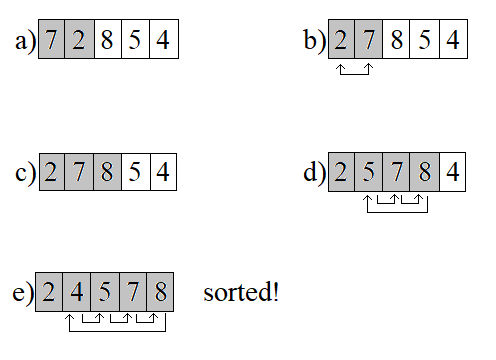
\includegraphics[scale=0.5]{insertion_sort}
\caption{
    The process of insertion sort. \textbf{(a)} Start with the first two values--7 and 2. \textbf{(b)} 2 and 7 are properly sorted. \textbf{(c)} Consider the third value, 8 is already greater than 7, so do not swap. \textbf{(d)} Consider the value 5, insert it after 2, which means iteratively swapping values towards the left to make room. \textbf{(e)} Place value 4 in between 2 and 5, adjust like in (d).
}
\label{fig:insertion_sort}
\end{figure}
\\ \\
Here is some pseudo code from the book (without comments), with $A$ being some array with $n$ values.

%------------------------------------------------
% Insertion sort
%------------------------------------------------
\begin{codebox}
\Procname{$\proc{insertion-sort}(A)$}
\li \For $j \gets 2$ \To $\attrib{A}{length}$
\li     \Do
            $\id{key} \gets A[j]$
\li         $i \gets j-1$
\li         \While $i > 0$ and $A[i] > \id{key}$
\li             \Do
                    $A[i + 1] = A[i]$
\li                 $i \gets i-1$
                \End
\li         $A[i+1] \gets \id{key}$
        \End
\end{codebox}

%================================================
\section*{Analysis of Insertion Sort}
%================================================
Writing pseudo code is neat and all, but it would be nice if we could understand its running time, below is how the book approaches tackling running time, and it displays it neatly. Simply put, write a cost for each line, and the number of times that line may run.
\\
\\
Line$\hspace{15mm}$Cost$\hspace{15mm}$Times$\hspace{15mm}$\\
1$\hspace{20mm}c_1$$\hspace{20mm}n$\\
2$\hspace{20mm}c_2$$\hspace{20mm}n - 1$\\
3$\hspace{20mm}c_3$$\hspace{20mm}n - 1$\\
4$\hspace{20mm}c_4$$\hspace{20mm}\sum_{j=2}^{n} t_j$\\
5$\hspace{20mm}c_5$$\hspace{20mm}\sum_{j=2}^{n} (t_j-1)$\\
6$\hspace{20mm}c_6$$\hspace{20mm}\sum_{j=2}^{n} (t_j-1)$\\
7$\hspace{20mm}c_7\hspace{20mm}n-1$\\
\\
On an input of n values, sum the products of the cost and times columns, this gives
\\
\\
\begin{multline*}
T(n) = c_1n + c_2(n-1) + c_3(n-1) + c_4\sum_{j=2}^{n} t_j + c_5\sum_{j=2}^{n} (t_j-1) + c_6\sum_{j=2}^{n} (t_j-1) + c_7(n-1)
\end{multline*}
\\
\\
For insertion sort, the best case occurs when the input is already sorted, giving
\\
\\
\begin{equation*}
\begin{split}
T(n) & = c_1n + c_2(n-1) + c_3(n-1) + c_4(n-1) + 0 + 0 + c_7(n-1) \\
  & = (c_1 + c_2 + c_3 + c_4 + c_7)n - (c_2 + c_3 + c_4 + c_7)
\end{split}
\end{equation*}
This can be expressed in the form $an + b$, and will give a best case running time of $\Theta(n)$.
\\
\\
The worst-case occurs when the input is in reverse-order, this gives
\begin{equation*}
\begin{split}
T(n) & = c_1n + c_2(n-1) + c_3(n-1) + c_4\sum_{j=2}^{n} t_j + c_5\sum_{j=2}^{n} (t_j-1) + c_6\sum_{j=2}^{n} (t_j-1) + c_7(n-1) \\
  & = c_1n + c_2(n-1) + c_3(n-1) + c_4\bigg(\frac{n(n+1)}{2} - 1 \bigg) + c_5\bigg(\frac{n(n-1)}{2}\bigg) + c_6\bigg(\frac{n(n-1)}{2}\bigg) + c_7(n-1) \\
  & = \bigg(\frac{c_4}{2} + \frac{c_5}{2} + \frac{c_6}{2}\bigg)n^2 + \bigg(c_1 + c_2 + c_3 + \frac{c_4}{2} - \frac{c_5}{2} - \frac{c_6}{2}\bigg)n - (c_2 + c_3 + c_4 + c_7)
\end{split}
\end{equation*}
This can be expressed as $an^2 + bn + c$, and will give the form of $\Theta(n^2)$, the worst case.

\end{document}
